\documentclass[dvipdfmx]{beamer}
\usetheme{metropolis}           % Use metropolis theme
\usepackage{float}
\usepackage{listings,jvlisting} %日本語のコメントアウトをする場合jvlisting(もしくはjlisting)が必要
%ここからソースコードの表示に関する設定
\lstset{
  basicstyle={\ttfamily},
  identifierstyle={\small},
  commentstyle={\smallitshape},
  keywordstyle={\small\bfseries},
  ndkeywordstyle={\small},
  stringstyle={\small\ttfamily},
  frame={tb},
  breaklines=true,
  columns=[l]{fullflexible},
  numbers=left,
  xrightmargin=0zw,
  xleftmargin=3zw,
  numberstyle={\scriptsize},
  stepnumber=1,
  numbersep=1zw,
  lineskip=-0.5ex
}

\title{Progress}
\date{\today}
\author{Mizuno Yasuaki}
%\institute{Centre for Modern Beamer Themes}
\begin{document}
  \maketitle
  
  \begin{frame}{目次}
    \begin{enumerate}
      \item プログラムの整理
      \item 少ないデータでの学習
    \end{enumerate}
  \end{frame}

  \begin{frame}{プログラムの整理}
    画像生成と機械学習のプログラムが散乱していたので整理した。
    \begin{itemize}
      \item generate\_img
      \begin{itemize}
        \item common
        \item prc
      \end{itemize}
      \item train\_img
      \begin{itemize}
        \item common
        \item prc
      \end{itemize}
    \end{itemize}
  \end{frame}

  \begin{frame}{プログラムの整理}
    改良
    \begin{itemize}
      \item 千個の画像データごとに保存し直した
      \item modelを生成し、コンパイルして返す関数の作成
    \end{itemize}
  \end{frame}

  \begin{frame}[fragile]{最も単純なFNNモデル生成}
    \begin{lstlisting}[caption=Simple\_FNN.py]
      def Simple_FNN(input_shape, output_shape):
        model = keras.Sequential([
            layers.Flatten(input_shape=input_shape),
            layers.Dense(128, activation='relu'),
            layers.Dense(output_shape)
        ])
        model.compile(
            optimizer='adam',
            loss=keras.losses.SparseCategoricalCrossentropy(from_logits=True),
            metrics=['accuracy']
        )
    
        return model
    \end{lstlisting}
  \end{frame}

  \begin{frame}{少ないデータでの学習\footnote{多くのデータを使うと使用メモリをオーバーするため}}
    \begin{itemize}
      \item 使用データ
      \begin{itemize}
        \item 訓練データ:30000
        \item テストデータ:6000
      \end{itemize}
      \item 使用したモデル
      \begin{itemize}
        \item 順伝播ニューラルネットワーク
        \item 畳み込みニューラルネットワーク
      \end{itemize}
    \end{itemize}
  \end{frame}

  \begin{frame}[fragile]{FNNによる学習}
    \begin{itemize}
      \item 使用モデル\mbox{}\\
        \begin{lstlisting}[caption=generate\_simple\_fnn.py]
          model = keras.Sequential([
            keras.layers.Flatten(input_shape=input_shape),
            keras.layers.Dense(128, activation='relu'),
            keras.layers.Dropout(dropout_ratio),
            keras.layers.Dense(output_shape)
          ])
        \end{lstlisting}
      \item ハイパーパラメータ\mbox{}\\
      \begin{itemize}
        \item optimizer='adam'
        \item dropout\_ratio=0.0
        \item epochs=30
      \end{itemize}
    \end{itemize}
  \end{frame}

  \begin{frame}{FNNによる学習学習結果}
    Test Accuracy: 0.28896206
    \begin{figure}[H]
      \centering
      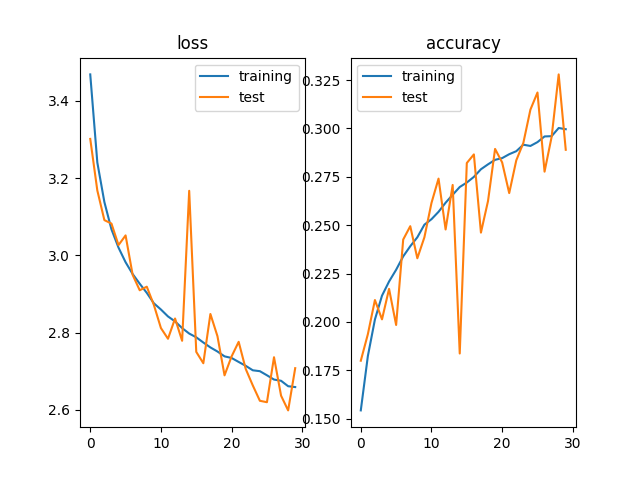
\includegraphics[keepaspectratio, scale=0.5]{images/train_fnn.png}
      \caption{result\_fnn.png}
    \end{figure}
  \end{frame}

  \begin{frame}[fragile]{CNNによる学習}
    \begin{itemize}
      \item 使用モデル\mbox{}\\
        \begin{lstlisting}[caption=generate\_simple\_fnn.py]
          model = keras.models.Sequential([
            keras.layers.Conv2D(32, (3, 3), activation='relu', input_shape=input_shape),
            keras.layers.MaxPooling2D((2, 2)),
            keras.layers.Flatten(),
            keras.layers.Dense(64, activation='relu'),
            keras.layers.Dropout(dropout_ratio),
            keras.layers.Dense(output_shape)
          ])
        \end{lstlisting}
      \item ハイパーパラメータ\mbox{}\\
      \begin{itemize}
        \item optimizer='adam'
        \item dropout\_ratio=0.0
        \item epochs=10
      \end{itemize}
    \end{itemize}
  \end{frame}  

  \begin{frame}{CNNによる学習学習結果}
    Test Accuracy: 0.87836062
    \begin{figure}[H]
      \centering
      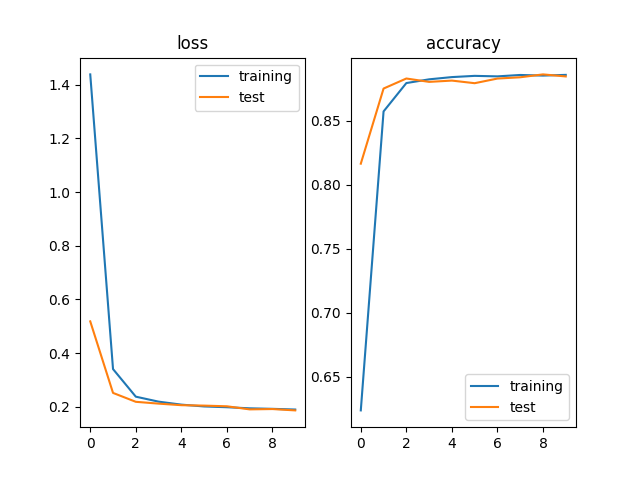
\includegraphics[keepaspectratio, scale=0.5]{images/train_cnn.png}
      \caption{result\_cnn.png}
    \end{figure}
  \end{frame}

  \begin{frame}{まとめ}
    \begin{itemize}
      \item CNNを使ったほうが精度\mbox{}\\
        より複雑なCNNを使って学習を進める
      \item 過学習はあまり見られなかった
      \item より最適なハイパーパラメータを探す
      \item 多くのデータを使用して学習する方法を模索する
    \end{itemize}
  \end{frame}
\end{document}

